%=== Part I - Foundations ===%
\part{Foundations}

\chapter{Introduction}
\section{Motivation and Problem Statement}

CPS team - waht do they need it for
code growing user base - interconnecticty os , other qualities speaking for the usage of vs code
-
already in possesion of Haskell Checker but

\label{sec:scope}
\section{Objectives and Scope}
The main goal of the thesis was to create a \textit{Language Extension} ?NAME? for \textit{MiniProb}. Language extensions are a big part of
VS Code’s extension ecosystem and enable the editor to utilize custom language tooling. Such extensions support the user during the implementation process
while writing code, by providing language assistance like syntax validation or code completion. While this implementation targets VS Code, the underlying
logic and functionality are not limited to it - through the use of the \textit{Language Server Protocol (LSP)}, the developed tooling can be reused across
various editors and IDEs that support the protocol. The core functionality of these extensions stems from \textit{parsers} which, against a formal language
definition, convert written text into abstracted parts, validating the code in the process. These parts can then be used to extend the capabilities of the
tooling to encompass referential validation, type checking, code completion, diagnostics, and other language services that enhance the development experience.

In order for parsers to function accordingly, they require formal language definitions or models. These definitions range from various types of grammars to
abstract machines such as automata, which together provide the structural and syntactic rules necessary for correct interpretation and validation of source code.
Based on these definitions, parsers are able to systematically identify the hierarchical structure of a program by recognizing patterns, token sequences, and nested
constructs, ensuring that the code adheres to the expected form before any further processing or analysis occurs.
In this thesis, a generative context-free grammar is used to formally describe \textit{MiniProb}, a domain-specific language (DSL) designed for authoring \textit{POMC} files.
With this grammar as a foundation, parsers enable the implementation of a fully functional language extension to aid developers writing POMC files.\\
Ultimately, the resulting extension, titled ?NAME?, is intended to provide comprehensive language support. This includes syntactic and semantic analysis
through syntax highlighting and validation, accurate resolution of symbol references and rudimentary code completion, as well as implemented type checking mechanisms
to ensure compatibility during development.

An appropriate set of regression tests was developed to ensure the continued correctness and stability of the language tooling.
These tests include parsing tests, which verify that valid input is correctly recognized and structured according to the grammar; validation tests,
which ensure that semantic rules are properly enforced and errors are accurately reported; and linking tests, which check that references between symbols
or declarations are correctly resolved across different parts of a program. Together, these test categories help maintain the integrity of the parser and language service as
the implementation evolves.

Lastly, this thesis includes an evaluation of the newly implemented parser, focusing on its correctness and performance in practical usage scenarios.
The evaluation is based on metrics collected from representative input samples, measuring factors such as parsing speed, memory usage, and error handling.
Where relevant, comparisons are also drawn against the existing \textit{Haskell}-based parser for \textit{.pomc} files, offering a point of reference to assess
improvements or trade-offs introduced by the new implementation.

\chapter{Background on Languages \& Grammars}

\label{sec:formallang}
\section{Formal Language Theory}

Formal language theory deals with the study of languages - sets of strings constructed from alphabets - and the formal grammars that determine and generate them.
In contrast to natural languages, which have evolved over centuries under the influence of diverse cultural, historical, and environmental factors,
formal languages do not inherently relate to any perceived constructs of our environments and are generally not intuitively understood.
Additionally, formal languages do not share the rich evolutionary progression - a lengthy process of gradual adaptations and refinements spanning generations -
of their natural counterparts. Instead, they employ sets of axiomatic \textit{production rules} that describe each language individually.
The field of formal language theory sprung from linguist Noam Chomsky's attempts during the 1950s to definitively characterize the structure of natural languages
using mathematical rules.\cite{Jiang_Li_Ravikumar_Regan_2009} This analytical approach led to development of the \textit{Chomsky hierarchy}, which proved
to be a vital theoretical foundation for later discoveries and applications, as it was found that all information(photos, videos, numbers, axioms) can be
represented as finite strings.\\

The \textit{Chomsky Hierarchy} is a hierarchical classification of formal grammars, that labels them to four groups. The grammars are ranked based on the
individual \textit{expressive power} of the languages they produce, with each class including the less expressive ones. The whole hierarchy consists of four
groups of grammars (and corresponding language classes), that are identified by inspecting the production rules, which get progressively less restrictive.

\textbf{Type-3} grammars, or \emph{regular} grammars, generate exactly the class of regular languages. Their productions are restricted to the two equivalent styles:
\[
  right-reg.: \quad A \;\to\; aB \quad or \quad A \;\to\; a
  \qquad and \qquad
  left-reg.: \quad A \;\to\; Ba \quad or \quad A \;\to\; a,
\]
where \(A,B\) are nonterminals and \(a\) is a terminal. Regular expressions provide an alternative, declarative notation for these languages - each expression
can be mechanically transformed into a regular grammar, and vice versa. More broadly, every grammar in the Chomsky hierarchy admits an equivalent acceptor automaton;
in the case of Type-3 grammars, this correspondence yields deterministic or nondeterministic finite automata. Leveraging these conversions makes regular grammars
invaluable in practice (for example, in lexical analysis, pattern matching, and protocol verification), even though their expressive power is the most limited.
\textbf{Type-2} grammars, or \emph{context-free} grammars (CFGs), produce all context-free languages.
Their rules take the general form  \[A \;\to\; \alpha\] where \(A\) is a single nonterminal and \(\alpha\) is any string of terminals and nonterminals.
This additional flexibility captures nested, hierarchical structures-like balanced parentheses or most programming‐language syntaxes - that regular grammars cannot.
Each CFG is accepted by a corresponding pushdown automaton: the grammar expansions map naturally onto push and pop operations on the PDA’s stack, making the grammar-automaton
equivalence at this level another cornerstone of formal language theory.

The thesis focuses on the above mentioned classes, as these are the ones applicable in the implementation part of the language service?NAME?. The last two classifications
\textbf{Type-1} and \textbf{Type-0} grammars, can create \textit{context-sensitive} and \textit{recursively enumerable} languages respectively, and are the most expressive
of all with Type-0 grammars placing absolutely no constraints on the production, making them only acceptable by Turing-Machine.

\subsection{Backus-Naur Form (BNF) and Variants}
Even though production rules, alphabet specifications, and automaton definitions suffice to unambiguously define the set of valid strings/sentences in a language, their notation
tends to be opaque and cumbersome in practice, prompting interest in forming intuitively comprehensible grammar definitions. The Backus-Naur Form (BNF),
created by John Backus with contributions by Peter Naur and released in their Algol-60 report\cite{ALGOL60}, was a pivotal introduction furnishing a concise, human-readable syntax for language generation.
By expressing each rule as
\[
  \langle\mathrm{nonterminal}\rangle \;::=\; expansion_1 \;|\; expansion_2 \;|\;\dots
\]
BNF allows both sequencing and alternation of multiple expansions, enabling language designers to articulate complex, nested structures while preserving structural
clarity and high readability.
This declarative approach not only supports rigorous specification but also facilitates mechanical parsing, thereby advancing the practice of compiler development and
language tooling.

While BNF provides a clear, formal way to describe language syntax, it suffers from verbosity and redundancy - pure BNF grammars often become bloated when encoding
common patterns like optionals or repetitions requiring auxiliary nonterminals for a sufficient description and, over time, has been extended and modified for various
use-cases spawning a new family of grammar notations. The \textbf{Extended Backus-Naur Form} extends BNF by adding more expressive meta-syntax, introducing operators
similar to \textit{Regular Expressions} allowing the use of optional or repeatable expressions, commonly indicated by brackets but not limited to '[\dots]' and '\{\dots\}',
and the use of comments. Such extensions make grammars more compact and easier to read without changing the fundamental class of languages they describe.
Multiple distinct instances of EBNF's have been development, all with minor syntactic differences, yet there really is no on-for-all EBNF used in practice, although
a standardized ISO/IEC 14977 version exists. \cite{jinks2004bnf,jinks2004ebnfvariants}\\
Within the scope of my thesis, \textit{?NAME?}, Extended Backus-Naur Form (EBNF) is particularly significant, since Langium employs its own custom EBNF dialect ?makeRefTo?
to define the grammars underpinning its language-assistance features. \ref{sec:langium-grammar}

\section{Language Structure and Paradigms}

\subsection{Parsing Models}

Parsing strategies play a central role in the implementation of programming languages, determining how source code is analyzed and transformed into syntax trees.
Two primary streams dominate the landscape: top-down and bottom-up parsing. Each parsing approach encompasses distinct implementation strategies and imposes specific
constraints on grammar design, thereby influencing the overall complexity of language implementation.

Top-down parsers, such as those following the \textit{LL($k$)} model, process input from left to right, constructing parse trees from the root downward.
These parsers require grammars to avoid \textit{left recursion}, a situation where a non-terminal refers to itself as the first symbol on the right-hand side of a
production (e.g., \texttt{A}~$\rightarrow$~\texttt{A}~$\alpha$). Left-recursive rules can lead to infinite recursion during top-down parsing.
In contrast, \textit{bottom-up} parsers, including \textit{LR($k$)} and its variants, build parse trees from leaves to root and can naturally accommodate
left-recursive structures.

The parameter k in LL(k) and LR(k) denotes the number of lookahead tokens needed to unambiguously select production rules.
Larger values of k allow more expressive grammars but may increase the complexity of the parser and slow down parsing.
As such, grammars used in practice are often simplified or transformed to be compatible with the limitations of the chosen parsing model.

Understanding these parsing models is crucial when designing or analyzing a programming language, especially when employing parser generators such as
ANTLR and Chevrotain (LL) or Yacc/Bison (LR), which impose specific requirements on grammar structure.

\subsubsection*{Lexers}
todo

\subsection{Abstract vs. Concrete Syntax}

The terms \textit{abstract} and \textit{concrete} syntax are primarily encountered in the context of programming language design. While the two concepts follow the common relationship of
abstract and concrete instances - where one embodies a generalized, meta-level blueprint, while the other encapsulates the concrete, instance-level details - and the term "syntax" broadly applies to all languages,
the idea of pinning meta-information onto language constructs, somewhat implies further calculations based on the language itself.

When designing programming languages, the abstract syntax is of particular interest, as its streamlined view of the language is ideally suited for developing
validation constraints or type systems and for general interpretation. This is done most commonly by encoding the syntax into a \textbf{Abstract Syntax Tree (AST)},
a tree-like structure containing nodes for each high-level construct (such as expressions, declarations, or statements) connected according to their logical hierarchy,
while deliberately omitting lexical details to yield a canonical. \cite{slonneger1995specifying}
The \textbf{Concrete Syntax Tree (CST)} is the specialized counterpart to the AST and consists of a full parse-tree, preserving every terminal and nonterminal
token(keywords, delimiters, etc.) and mirrors each grammar production in its node structure, providing the complete syntactic context possibly needed for precise error
reporting and tooling. \cite{aho2006compilers}

\label{sec:prog-paradigms}
\subsection{Imperative vs.\ Declarative Languages}

Languages used for further computation can be analyzed from multiple perspectives and classified with different qualities in mind. \cite{progParadigmsForDummiess}
For this thesis we focus on slotting languages into two overarching paradigms, \textbf{imperative} and \textbf{declarative} languages,
which differ primarily in how they express the path toward a desired outcome.
Declarative languages describe \textit{what} the computation should accomplish by adhering to sets of expressions, constraints or logical statements. \cite{grammarDrivenDSLDebug}
These formulas set the rules and goals characterizing the desired result or relationship of input and output values. The actual control flow and low-level decisions of
the execution is left to the specific language implementations and runtime engines.

\begin{figure}[ht]
  \centering
  \begin{forest}
    for tree={
    draw,
    rounded corners,
    align=center,
    parent anchor=south,
    child anchor=north,
    grow'=south,
    l sep=15pt,
    s sep=10pt,
    }
    [Programming Paradigms
      [Imperative
          [Procedural]
          [Object-Oriented]
          [Parallel]
      ]
      [Declarative
          [Logic]
          [Functional]
          [Database]
      ]
    ]
  \end{forest}
  \caption{Commonly encountered programming paradigms.}
  \label{fig:programming-paradigms}
\end{figure}

Generally, because of the vague wording used, the paradigms themselves are not always completely and accurately describing the behaviour of a programming language,
possibly leading to different concepts overlapping. This is especially clear in modern languages, which often implement functionality by borrowing
constructs from the opposite paradigm - for example, imperative C\# incorporates declarative features through its LINQ-Library, while Haskell, functional by
design, supports imperative-style programming.\\

Imperative languages, in contrast to declarative ones, describe \textit{how} a computation will accomplish the desired end-state by following explicit sequences
of commands. These commands consist of statements that actively manipulate the computations state, which is typically managed through assignments to variables
and taking charge of the control flow with provided language constructs (loops, conditionals, calls, procedures, etc.).
Consequently, correct execution is no longer responsibility of the underlying system, but the implementation and therefore the programmer themselves. The imperative paradigm
reflects von Neuman machines - accessing memory and hardware directly. This fined grained control enables the use of low-level optimization techniques \cite{lowLvelOpt}.
As programmers instruct the machine how to do something, certain performance characteristics and resource constraints can be impelled depending on the context of the computation.
Such techniques encompass memory and cache management, \textit{Instruction-Set} optimization or compiler optimization.

However, while this explicit control provides developers with great functional freedom, it also places a greater burden on them to manage every detail of execution.
Because the programmer must specify each step - from how data is stored in memory to the order in which operations occur - imperative code can become verbose and cluttered obscuring the high-level intent.
Moreover, mutable state and side effects introduce the risk of subtle bugs, especially in concurrent or parallel settings where unintended interactions between state changes
can lead to race conditions. Also, formal reasoning and verification are more complex, since proving correctness requires tracking every state
transition rather than relying on \textit{referentially transparent} expressions.

Typical use cases for imperative programming include algorithmic or process-oriented problems where an explicit series of steps is natural.
Low-level system programming, embedded development, and performance-sensitive routines frequently rely on imperative constructs to manage hardware resources directly.More actions
In scenarios that demand fine-grained stateful interactions - such as updating user interfaces incrementally, reading and writing files in a specific order, or
controlling physical systems via commands - imperative languages shine by giving developers precise command over execution.
Simulation engines, game logic, and scripting or “recipe”-style automation languages also favor imperatively describing each step to achieve the desired outcome.

\section{Domain-Specific Languages (DSLs)}

Domain-Specific languages are programming or specification languages which are tailored to specific application domain, providing constructs and abstractions
that capture the domain concepts. \cite{whenHowDSL} In stark contrast to general-purpose languages (GLPs) that aim for broad applicability, a DSL waives generality in favor
of higher expressive power in its domain of interest. By offering notation closely related to a domains phrasing, a DSL allows solutions to be formulated at the same level
of abstraction as the domain itself, mapping language primitives onto the domain concepts. Developers, therefore, are able to create programs or specifications more
productively and securely.

The close relationship of DSL and domain furnishes multiple advantages over conventional GLPs: it reduces the amount of general programming knowledge needed,
expanding the pool of developers from traditional programmers to also domain experts. Moreover, DSLs declutter code, rather than describing a subproblem of the domain
with multiple lines of code, fewer are needed because constructs inherently carry domain specific information, also contributing to broader comprehensibility for those familiar with the domain.
DSLs solutions are also easier to formally verify, as they are restricted to a limited context, than GLPs for which proving correctness is extremely hard.

However, DSLs can suffer from limited scope and flexibility even within their target domain, forcing developers to fall back on general-purpose languages when they need functionality outside the
DSL's narrow focus. Furthermore, if the domain itself is complex or rapidly evolving, creating and maintaining a DSL may still demand deep domain expertise, because the abstractions must
accurately capture all necessary domain rules and nuances.

\subsection{Imperative DSLs}

Whichever paradigm a DSL follows is mostly guided by the specifics of the domain to describe. Even though DSLs usually adhere to a declarative approach \cite{sigplanDSL}, which follows from a
major motivation: wanting to describe \textit{what} is expected of the domain in high-level abstraction, a domain may emit qualities that invoke more imperative thinking.
If the nature of a domain is inherently composed of sequential actions, consists of procedures or stateful operations, the imperative paradigm is more appropriate.
Imperative DSLs require the user to script solutions in step-by-step fashion using domain-specific commands and statements. Essentially,the user embeds domain concepts as a sequential programming model,
where the control flow and state transitions of the domain computations have to be managed.

In domains where fine-grained control and explicit ordering matter, imperative DSLs provide maximal flexibility, because every aspect of the execution is adjustable.
This level of control becomes crucial when timing or order of operations yield different outcomes, or when fine-tuned performance optimizations are required.
Furthermore, building an applicable imperative DSL is often simpler than creating a declarative one: an interpreter processes each command in sequence,
or a translator converts DSL instructions into a host general-purpose language.

Imperative DSLs are well suited for scripting and defining macros, where users sequence domain-specific commands to drive behavior. They also shine in combination with testing
frameworks and scenario specifications, where user interfaces describe interactions by specifying a timely sequence of user inputs. In robotics and industrial automation,
imperative DSLs allow to program custom action sequences - such as picking up an object, then placing it - where each step must follow a
strict order to ensure safety and accuracy. More broadly, any process-control domain that relies on precise sequencing and stateful interactions benefits from the clarity
and control that an imperative DSL provides.

\chapter{Cyber-Physical Systems and Formal Analysis}

\section{Cyber-Physical Systems: Definition and Examples}

Cyber-Physical System (CPS) is an umbrella term broadly referring to any systems which tightly integrate both computational logic (cyber) and physical components, allowing interplay
through designated interfaces. \cite{cpsModelDesc} The two parts of a CPS have to be seamlessly interconnected enabling efficient communication and consistent information
relying?? \cite{cpsChallengesAndFuture}, as both sides heavily depend on one another.
The cyber-physical relationship can be generally describes by three roles \textit{controller/agent}, \textit{sensors} and \textit{activators},
which are connected by an underlying network.
Controllers, representing the 'cyber', are occupied with computation and relying fitting instructions based on te observational data provided by the physical sensors.
Sensor and Actuators embody the 'physical' and are the ones interacting with the environments in which the system resides. A sensors jobs is to gather intel from its
surroundings communicating it in order for the agent to make correct decisions and predictions and to monitor the system. Without sufficient data, the controller is left
blind and possibly  unable to perform as intended. While sensors passively interact with the environment by observing, actuators do so actively by altering the systems state
- carrying out tasks instructed by the controller. This sense->compute->actuate cycle is executed iteratively, forming a continuous feedback loop that enables the system to
respond dynamically to changes in its physical environment.

\begin{figure}[htbp]
  \centering
  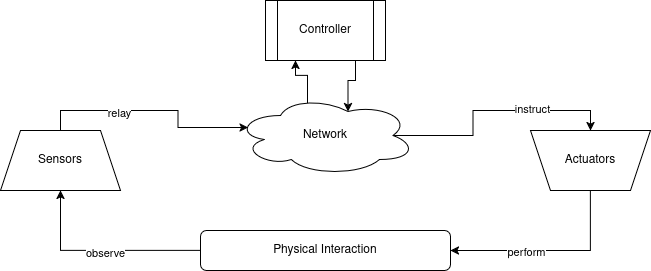
\includegraphics[width=0.7\textwidth]{graphics/cpsGeneralArchitecture.png}
  \caption{General architecture of common CPS}
  \label{fig:cps_architecture}
\end{figure}


Controllers may range from simple reactive routines to advanced inference models grounded in probabilistic programming, or even intelligent agents capable of autonomous
decision-making. Actuators, in turn, translating these decisions into physical action can be represented by basic devices such as motors that move parts,
valves that regulate flow, or relays that control circuits. They can also act as more complex assemblies - robotic joints, programmable hydraulic systems, or smart actuators
that adjust based on local conditions. At the foundation, sensors continuously monitor the environment, capturing data through modalities such as motion,
orientation, or spatial mapping. Together, these elements form  an integrated feedback system, enabling CPS to respond intelligently and flexibly to their physical context,
regardless of application domain.\\

CP-Systems are inherently multidisciplinary structures intersecting engineering domains (mechanical, electrical, civil, etc.) with computer science.
Because these domains employ differing models for ... , effectively combining them is non-trivial. Challenges arise during development and operation of CPSs for which
finding solutions is imperative. \cite{cpsChallengesAndFuture} First and foremost is the concern of \textbf{reliability and safety}. Occurrences of failures can have dire real-world
consequences with catastrophic end results. This means systems must handle unexpected conditions gracefully and robustly. But ensuring safety through extensive verification
and validation is complicated by the combination of continuous physical dynamics and discrete decision logics. Another challenge is \textbf{real-time performance}, as computing
elements must keep pace with the physical processes, which usually require low-latency responsiveness including the network. Since CPSs are used in infrastructure and other
critical sites that may be targets of cyber attacks, guarantying a high standard of \textbf{Security} is essential. Additionally, sensors are not completely reliable -
possibly introducing noise to measurements - and environmental conditions can vary drastically leading to \textbf{uncertainty}, which a CPS has to cope with to be resilient. \cite{cpsProbabilisticRobotics}

\label{sec:formal-methods}
\section{Formal Methods and Model Checking}

CPSs are often deployed in safety-critical environments where utmost importance is placed on reliable operation and functional correctness. Yet reaching high levels of confidence
in a systems behavior remains extremely inside cyber-physical domains.\cite{formalMethodsCPSCritical} This difficulty arises from the complex interactions of all the individual integral
components of the system, which can not be effectively tested only employing traditional methods. The inherent entanglement of these systems warrants the use of
specialized procedures that are able to cover and validate the acting components. Unlike conventional simulation based testing, \textit{formal methods} are able to prove correctness against
formal specifications, thereby providing more reliable results and eliminating potential error sources, such as race conditions or violations of safety properties(unnoticed states).

In formal methods, \textit{theorem proving}, \textit{model checking}, and \textit{runtime verification} are widely recognized as the three main approaches for assuring
system correctness\cite{formalMethodsBig3,formalMethodsCPSCritical}.
All three practices are distinguishable from one another and are tailored for certain scenarios. Runtime verification is a lightweight technique that verifies systems
by inspecting their execution trace - often employing automata to detect violations. Theorem proving, in contrast, is an offline and often time intensive
process relying on mathematical inference rules to statically validate correctness with a high degree of rigor.\\

Model checking is of most interest in this case, as the MiniProb DSL \ref{sec:miniprob} was developed with this context in mind. \cite{POPACheck}
It statically verifies a system by exhaustively exploring the state-space and is considered one of the most successful verification techniques. \cite{formalMethodsCPSCritical}
The thorough analysis of reachable states, combined with specifications which are expressible in various forms of modal logic,
offer a strong expressive foundation for property verification \cite{modelCheckingPrinceples}. However, the systematic exploration of states leads to poor performance, especially for model with
complex and big state spaces. Moreover, as most model checking implementation employ automata-based solutions, systems are usually converted into
equivalent state machines which can result in an explosion of states.\cite{}
Model checking is generally only used in conjunction with finite-state machines for aforementioned reasons. Still, theres been advances trying to apply it to infinite state spaces.
\cite{modelCheckingInfCounter,modelCheckingInfSymb}. The resulting verdicts for infinite-state models are typically approximations or are restricted by bounded analysis,
such as checking only a finite number of steps or abstracting unbounded data domains. As a result, the verification outcomes may not provide absolute guarantees for all
possible executions, but rather assurances that hold under specific assumptions, abstractions, or within predefined limits of a system's behavior.

These approaches often rely on \textit{symbolic evaluation} rather than naive enumeration of states. By representing potentially infinite sets of states using logical
formulas or data structures such as Binary Decision Diagrams (BDDs) or SMT formulas, symbolic model checking can reason about system behavior without explicitly
generating every state.

\section{Motivation for PPLs in CPS Contexts}

Probabilistic programming has multiple fitting applications within CPSs, especially where reasoning under uncertainty is essential. Generally, probabilistic programming
allows controllers to plan even in unpredictable environments and settings.

\begin{multicols}{2}
  When measurements contain noise or are incorrect, PPL models can still be applied to extract useful information. Instead of treating the raw reading of a sensor as the “truth,”
  the readings are considered samples for a \textit{sensor’s model}. Not only is it possible to reduce the noise in the measurements by calculating the posterior,
  but those noise characteristics are also used to flesh out the predictive model itself.
  This enables PPLs to adaptively adjust noise models online when, for example, sensors deteriorate over time.
  Additionally - with most CPSs employing multiple sensors - a PPL naturally supports \textit{sensor fusion}, \cite{cpsSensorFusion} combining data from heterogeneous sources
  to produce a coherent estimate. By defining each sensor's observation as a conditional distribution, a probabilistic program
  weights each reading according to its uncertainty: more reliable sensors contribute more heavily, while inconsistent or faulty readings are down-weighted or flagged.
  Inference then yields a joint posterior over the true state, allowing the system to reconcile disagreements between sensors, detect potential sensor failures by inferring
  latent bias variables, and maintain a quantified confidence.
  \\
  Which leads us into robotics, a quintessential cornerstone of CPS. Instead of working on raw observational data and making assumptions in incomplete cases, robots can adopt
  a \textit{belief} based on an observational model \cite{cpsProbabilisticRobotics}. The observational model couples motion dynamics (how actions translate into state
  transitions) with existing sensor models, providing a full posterior distribution that the robot can use to imply different levels of confidence for its actions.
  Furthermore, robots often operate in changing environments or with components that degrade over time. Within a PPL, unknown parameters, such as friction
  coefficients or sensor calibration offsets, can be treated as latent variables and perform Bayesian learning to infer them from incoming data. The same inference mechanism used for state
  estimation thus also adapts the model online, continuously refining both motion dynamics and sensor mappings.
  \\
  A PPL expresses system dynamics probabilistically so that sampling yields a distribution of possible futures. \cite{cpsPredictiveControl} By enforcing “chance constraints”
  (e.g., “limit the probability of exceeding a safety threshold to 1\%”), inference or Monte Carlo sampling identifies control inputs that optimize expected performance while
  respecting risk. When the current state is uncertain, planning occurs in belief space - each action triggers a Bayesian update of the state distribution, and planners
  choose sequences that minimize expected cost given that uncertainty. Simultaneously, online Bayesian learning refines model parameters (like friction or drag) over time,
  tightening future predictions; as uncertainty shrinks, control can push closer to limits, whereas rising uncertainty leads to more conservative actions.
  \\
  Recent research is looking at ways to utilize PPLs to gather diagnostics of a CPS. \cite{cpsPPLDiagnostics} They authors propose a way to infer potential error causes, that
  might be overlooked otherwise, due to the .
  This of of great interest to system operators for deciding if either parts have to be replaced or only have to be recelebrated. Because measured data on system deviations
  often reflects complex intertwining causes and \textit{closed-loop corrections}, identifying root causes becomes a matter of inference. The proposed two-step approach
  first builds a generative model (based on control software and expert insights) that simulates observations from hypothesized error causes. This simulator is then recast
  as a probabilistic program, allowing Bayesian inference to estimate latent causes (with confidence intervals) from actual measurements.

\end{multicols}

\label{sec:pp}
\chapter{Probabilistic Programming}
\section{What Is Probabilistic Programming?}

Probabilistic programming is a paradigm that aims to perform statistical analysis using tools yielded by computer science.\cite{introductionprobabilisticprogramming}
Unifying general-purpose programming and probabilistic modelling enables the presentation of statistical models as a program. Defined by underlying program code, the model is
embodied by the relations between variables and calculations. The established capabilities of programming languages are often augmented with
probabilistic functionality, in ... creating probabilistic programming languages (PPL),\cite{probProgrammingPrinciples,2025modelcheckingprobabilisticoperator}
that are closely associated with this paradigm.
The enriched syntax enables the creation of more compact models and fosters conciser abstractions of the underlying probabilistic structure, usually providing constructs
that allow declaring random variables and conditioning of observed data. These primitives form the foundation for specifying core elements
of statistical models. \textit{Priors} are pre-known and usually drawn from distributions reflecting the initial belief over what value
\textit{latent variables}/model parameters might take on. \textit{Likelihoods} are also known beforehand representing how data is assumed to be generated given the
latent variable for which the \textit{posterior} is to be inferred. Together, these components form the backbone of a probabilistic model and provide the information required
to compute the posterior distribution, which is grounded in \textbf{Bayesian theory}.\cite{introductionprobabilisticprogramming}
\\

\textit{Bayes’ Theorem} provides the foundational framework for probabilistic reasoning under uncertainty. It describes how to update prior beliefs about unknown
quantities - known as latent variables - based on new evidence, resulting in a posterior distribution. Formally, it states that the posterior is proportional to the
product of the prior and the likelihood:
\[
  P(\theta \mid x) \propto P(x \mid \theta) \cdot P(\theta)
\]
In probabilistic programming, this principle is applied through models that define prior distributions over latent variables and likelihood functions for
observed data. The probabilistic programming language then applies Bayes' Theorem, typically via automated inference algorithms, to compute or approximate the posterior.
This makes it possible to express complex probabilistic models declaratively, while delegating the computation of posterior beliefs to the underlying inference engine.
\\

\section{Inference and Sampling Methods}

Inference is the process by which probabilistic models are "executed". Given a model and observed data, the task is to compute the posterior distributions of latent variables.
Because probabilistic models often include uncertainty and hidden variables, inference is the process that turns the model into concrete answers.
This process is abstracted and automated, but remains computationally nontrivial. Standard approaches to inference are generally grouped
into three main categories- \textit{exact inference}, \textit{sampling-based methods}, and \textit{variational inference}.\cite{bishop2006prml, blei2017vi, goodman2014dippl}.

\subsection*{1. Exact Inference}

Exact inference computes the posterior distribution analytically or through complete enumeration. This is possible only in models with limited complexity where the
entire state space can be traversed. Although conceptually straightforward, exact inference quickly becomes infeasible as model size increases, due to the combinatorial
explosion of possible states.

\subsection*{2. Sampling-Based Inference}

Sampling-based inference approximates the posterior by drawing samples from it, typically using Markov Chain Monte Carlo (MCMC) methods.
Continuously, random samples are generated from a given distribution - usually the prior or a conditional- and used to progressively approximate
the posterior with the model being executed repeatedly.
These approaches are flexible and can handle complex models, but they are often computationally expensive and require many samples to ensure accuracy.
The resulting samples can then be used to estimate expectations, marginal distributions, or event probabilities.

\subsection*{3. Variational Inference}

Variational inference formulates inference as an optimization problem. Instead of sampling, it produces a family of approximate distributions and seeks the member that
is closest to the true posterior. This involves defining an objective function - often the \textit{evidence lower bound (ELBO)} - and optimizing it using gradient-based methods.
Variational inference tends to be faster and more scalable than sampling, though it trades off exactness for speed by approximating the posterior rather than sampling
from it directly \cite{blei2017vi}.


\begin{figure}[htbp]
  \centering
  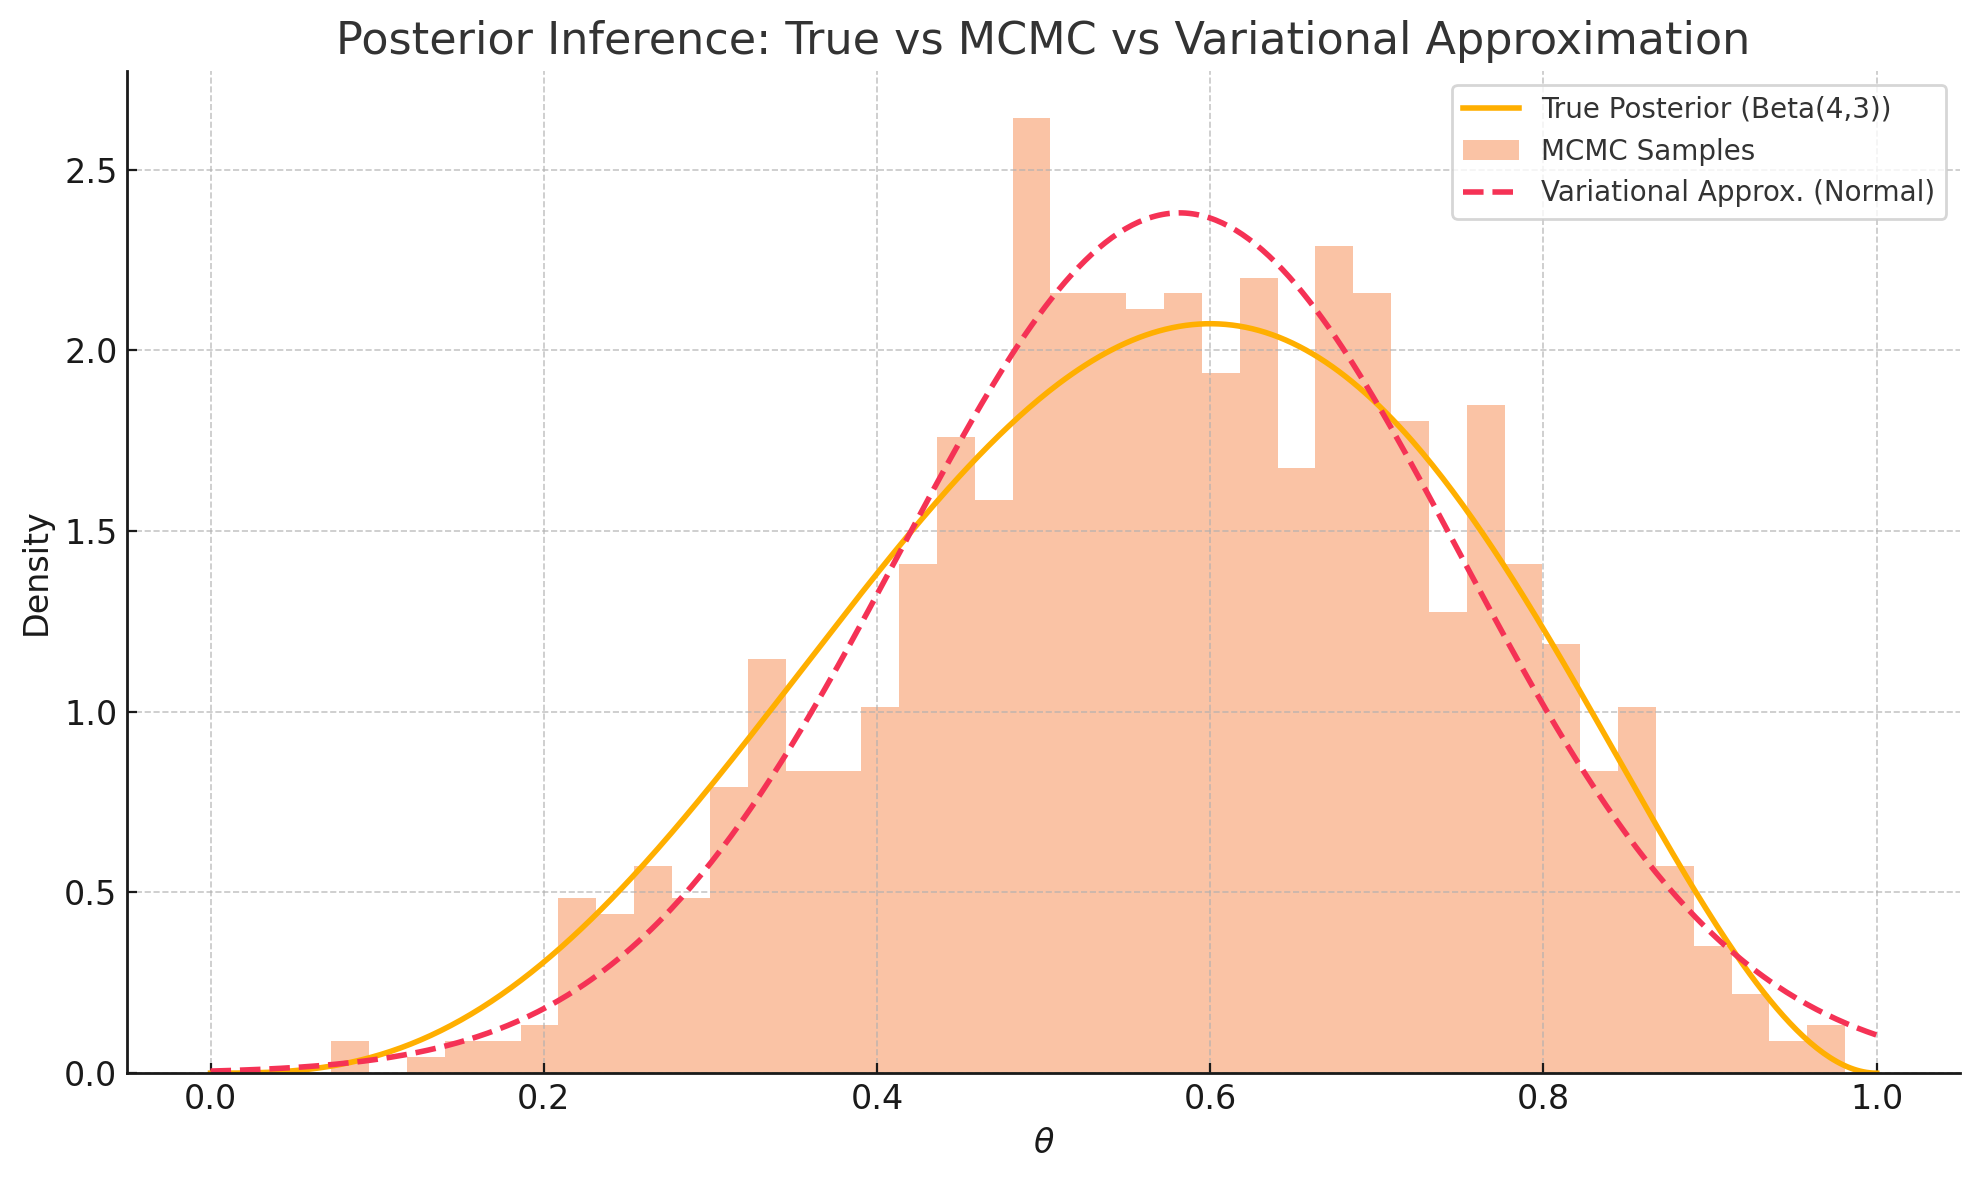
\includegraphics[width=0.7\textwidth]{graphics/inferencePlot.png}
  \caption{Comparison sample of exact posterior to inference methods}
  \label{fig:inference_plot}
\end{figure}

\section{Symbolic Semantics and Model Checking}

While probabilistic programming is typically associated with statistical inference and sampling-based evaluation, there exists an alternative perspective
that treats probabilistic programs as formal models subject to verification \cite{2025modelcheckingprobabilisticoperator,sato2019formal} as described in \ref{sec:formal-methods}.
In contrast to traditional inference, symbolic evaluation and model checking aim to rigorously analyze all possible executions of a program against formal specifications.

Symbolic approaches differ in that they do not enumerate individual executions or samples, but instead reason over entire sets of possible states and paths using
abstract representations. This enables analysis of program behavior in a more in-depth and automated way, making it possible to answer questions like:
“Does this property always hold, regardless of sampling outcomes?” or “What is the probability that this condition is eventually satisfied?”

Such techniques are particularly relevant for verifying probabilistic systems where correctness, safety, or reachability must be guaranteed rather than estimated.
They also enable reasoning about programs that would be challenging to analyze through sampling alone, such as those involving recursion, nondeterminism, or infinite state
spaces.

A growing body of foundational work has explored how symbolic and model checking techniques can be adapted to probabilistic
settings \cite{BaierClarkeHartonasGarmhausenKwiatkowskaRyan1997,EsparzaKuceraMayr2006,EtessamiYannakakis2012}. This includes approaches based on probabilistic automata, logics for probabilistic reasoning, and
symbolic representations of state spaces.

Building upon these foundations, the POPACheck tool \cite{POPACheck} represents a pioneering approach to verifying probabilistic programs with recursive structure.
By translating programs into probabilistic operator precedence automata - a formal model that can represent infinite state spaces - POPACheck allows for the analysis
of properties expressed in structured temporal logics. This enables verification of systems that lie beyond the scope of most traditional probabilistic programming
frameworks.

In this context, \emph{MiniProb} is used not for inference, but as a front-end language for describing probabilistic behavior that is ultimately verified through
model checking. The distinction between sampling-based execution and symbolic verification is presented below.

\section{Methodological Comparison}
\begin{table}[h]
  \centering
  \caption{Comparison of Probabilistic Programming in Traditional Inference vs. Formal Verification}
  \begin{tabular}{|p{4.5cm}|p{5.5cm}|p{5.5cm}|}
    \hline
    \textbf{Aspect}           & \textbf{Traditional Inference (e.g., Bayesian Modeling)}                      & \textbf{Formal Verification (e.g., Model Checking)}                                    \\
    \hline
    Primary Goal              & Estimate posterior distributions over variables (e.g., $P(\theta \mid data)$) & Prove correctness properties about probabilistic behavior (e.g., reachability, safety) \\
    \hline
    Evaluation Strategy       & Sampling-based execution (e.g., MCMC, SMC, VI)                                & Symbolic or exhaustive exploration of probabilistic state space                        \\
    \hline
    Execution Semantics       & Program runs as a simulator; samples are drawn during execution               & Program is interpreted mathematically; all behaviors are analyzed systematically       \\
    \hline
    Handling of Randomness    & Uses actual draws from distributions during execution                         & Treats random variables symbolically or via full enumeration                           \\
    \hline
    Output                    & Posterior samples, estimates, and confidence intervals                        & Probabilistic bounds, expected values, or formally verified properties                 \\
    \hline
    Typical Model Assumptions & Often uses continuous distributions and models real-world noise               & Often restricted to discrete, well-defined models for tractability                     \\
    \hline
    Result Guarantees         & Approximate; dependent on convergence and diagnostics                         & Sound (and often complete) within model and logic constraints                          \\
    \hline
  \end{tabular}
  \label{tab:inference_vs_verification}
\end{table}


\label{sec:miniprob}
\chapter{The \textit{MiniProb} DSL}
\section{Domain and Purpose}
\textit{MIniProb} is the successor of a DSL first introduced as \textit{MiniProc}\cite{miniproc}. Originally lacking the typical probabilistic
primitives such as \code{observe} and \code{query}, the language was designed for formal verification of recursive programs (see: \ref{sec:formal-methods}). As MiniProc focuses on recursive control-flow and
call-return semantics - qualities representative of procedural programming - it classifies under the imperative paradigm (see \ref{sec:prog-paradigms}). Furthermore, it is a
context-free language, since its structure is tightly coupled with the theory of \textbf{Operator Precedence Languages (OPLs)}, a deterministic subclass of CFLs (see: \ref{sec:formallangs}).
Programs written in MiniProc can be directly compiled into \textbf{Operator Precedence Automata (OPA)}, which leverage the structured nesting of procedure calls and
returns, thus enabling automata-based model checking via the \textit{POMC} tool against specifications written in the Precedence-Oriented Temporal Logic (POTL) \cite{miniproc}.
This conversions is made possible because MiniProc constraints its syntax to comply with the \textit{precedence relations} defined by a given
\textbf{Operator Precedence Matrix (OPM)}, allowing for deterministic and unambiguous parsing.
??MAKE SHORTER (note) same for PTLfx below??
\marginpar{}
\\

MiniProb extends MiniProc by incorporating primitives from PPLs \cite{POPACheck}, which enable sampling, conditioning and nested inference (see: \ref{sec:pp}).
While remaining recursive-procedural, it now belonging to the family of probabilistic programming languages, still within the context-free class, but no longer parsable to an OPA.
However, with the introduction of non-determinism and probabilistic transitions, MiniProb programs are able to be translated into
\textbf{probabilistic Operator Precedence  Automata (pOPA)} \cite{POPACheck,2025modelcheckingprobabilisticoperator}, that can represent both stack and stochastic behavior.
This transition enables formal verification of MiniProb programs via model checking, supporting \emph{qualitative}, \emph{quantitative}, and \emph{approximate} queries,
allowing to check whether properties - specified in $POTLf_\chi$ - hold with certainty, compute exact satisfaction probabilities, or obtain estimated bounds when exact computation is infeasible \cite{guideMiniProb}.

\begin{quote}
  POTL is a temporal logic specifically designed to express properties over Operator Precedence Languages (OPLs) \cite{chiari2020potlfirstordercompletetemporal,Chiari_2022}.
  Extending LTL, it includes modalities that refer to the hierarchical structure induced by procedure calls and returns,
  enabling formal reasoning about context-sensitive behaviors such as matching call-return sequences, stack inspection, and structured exception handling.
  The fragment POTL\textsubscript{$f_\chi$} restricts the logic to a form suitable for model checking over non-deterministic and probabilistic systems - particularly when
  used with probabilistic Operator Precedence Automata (pOPAs) - while retaining the expressive power needed to reason about structured control flows \cite{2025modelcheckingprobabilisticoperator}.
\end{quote}

MiniProb also incorporates expressing higher-order reasoning patterns, such as those involving mutually recursive queries that simulate agents reasoning about each other's
beliefs or decisions - a feature common in cognitive modeling and multi-agent systems \cite{multiAgent}.

As a DSL, MiniProb is not intended to offer the general-purpose capabilities of mainstream languages. In particular, it is not Turing-complete:
it lacks features like unbounded memory manipulation, arbitrary recursion without termination guarantees, or dynamic data structures. Its constructs are deliberately
limited to ensure compatibility with pOPA translation and to preserve decidability of model checking, which would not be possible in a fully general computational model.
\\

Ultimately, the purpose behind both MiniProc and MiniProb is to offer a high-level, user-friendly interface for programmers wishing to verify properties of recursive (probabilistic) programs without needing to manually translate their source code into OPA or pOPA representations. These DSLs thus serve as a crucial bridge between real-world programming constructs and the formal models required for rigorous verification.

\section{Syntax}

\begin{wrapfigure}{l}{0.5\textwidth}
  \centering
  \[
    \begin{array}{rcl}
      prog
       & \to  & (decl\;\texttt{;})^* \;func^+                                                     \\[6pt]

      decl
       & \to  & type\;\mathit{id}\;(\texttt{,}\;\mathit{id})^*                                    \\[6pt]

      func
       & \to  & \mathit{id}\;\texttt{(}
      (\,type\;\texttt{\&}?\;\mathit{id}
      (\texttt{,}\;type\;\texttt{\&}?\;\mathit{id})^*\,)?
      \texttt{)}                                                                                  \\[-2pt]
       &      & \texttt{\{}(decl\;\texttt{;})^*\;stmt^+\texttt{\}}                                \\[6pt]

      fcall
       & \to  & \mathit{id}\;\texttt{(}
      [\,e\;(\texttt{,}\;e)^*\,]
      \texttt{)}                                                                                  \\[6pt]

      stmt
       & \to  & lval\;\texttt{=}\;e\;\texttt{;}                                                   \\[-2pt]
       & \mid & lval\;\texttt{=}\;\texttt{Distribution(...)}\;\texttt{;}                          \\[-2pt]
       & \mid & (\texttt{query})?\;fcall\;\texttt{;}                                              \\[-2pt]
       & \mid & \texttt{observe}\;e\;\texttt{;}                                                   \\[-2pt]
       & \mid & \texttt{throw}\;\texttt{;}                                                        \\[-2pt]
       & \mid & \texttt{if}\;\texttt{(}e\texttt{)}\;\{\;stmt^*\;\}\;\texttt{else}\;\{\;stmt^*\;\} \\[-2pt]
       & \mid & \texttt{while}\;\texttt{(}e\texttt{)}\;\{\;stmt^*\;\}                             \\[-2pt]
       & \mid & \texttt{try}\;\{\;stmt^*\;\}\;\texttt{catch}\;\{\;stmt^*\;\}                      \\[6pt]

      lval
       & \to  & \mathit{id}\;(\texttt{[}e\texttt{]})?                                             \\[6pt]

      type
       & \to  & \texttt{bool}
      \;\mid\;(s\mid u)\;int\;(\texttt{[}int\texttt{]})?                                          \\[6pt]
    \end{array}
  \]
  \caption{Compacted grammar of \texttt{MiniProb}.}
  \label{fig:ebnf_grammar}
\end{wrapfigure}

??reference to BNF of MiniPRob from BNF section??

A compacted grammar for MiniProb is shown in \ref{fig:ebnf_grammar} containing the core elements for intuitive comprehension.
A full BNF grammar can be found in the appendix see \ref{fig:bnf_grammar}.
A \emph{prog} consists of zero or more top-level declarations followed by one or more function definitions. Each \emph{decl} introduces one or more variables of a
given \emph{type}, which may be \code{bool}, signed (\code{s}) or unsigned (\code{u}) integers of certain bit-width (e.g., \code{s8}, \code{u16}),
and optionally fixed-size arrays (e.g., \code{u8[10u4]}). Functions (\emph{func}) consist of an identifier, an optional list of typed parameters (passed by value or
reference via \code{\&}), and a block containing optional local declarations and at least one statement.

Within function bodies, MiniProb allows for local declarations and familiar C-like statements, including variable assignments (\code{lval = \emph{e};}),
function calls, and control flow structures such as \code{if}/\code{else}, \code{while} loops, and structured exception handling via \code{try}/\code{catch},
with \code{throw;} used to abort execution. Left-hand values (\emph{lval}) may refer to scalar variables or indexed array elements, while types follow a compact
convention, consisting of Booleans and signed or unsigned integers of fixed width.

Probabilistic constructs are central to MiniProb's design. These include sampling from distributions via statements like \code{lval = Distribution(...);},
currently supporting both \code{Bernoulli} and \code{Uniform} distributions. The \code{observe \emph{e};} construct allows conditioning execution on logical expressions,
rejecting traces that do not satisfy the observed condition. Inference is triggered through the \code{query \emph{fcall};} statement, which indicates
the probability evaluation of a function's outcome given a set of observations.

In addition to structured control, MiniProb supports expressions built from literals, variables, and function calls, composed using arithmetic
operations (\code{+}, \code{-}, \code{*}, \code{/}, \code{\%}), comparison operators (\code{==}, \code{!=}, \code{<}, \code{<=}, etc.), and Boolean connectives
(\code{!}, \code{\&\&}, \code{||}). These expressions can appear on the right-hand side of assignments or as arguments.

Beyond the standards, MiniProb introduces \emph{probabilistic assignments} to express uncertain choices: $lval = e_1 \{ e_2 : e_3 \} \; e_4$.
This construct selects $e_1$ with probability $p = e_2 / e_3$, and $e_4$ with probability $1 - p$.
Multiple such choice blocks can be chained to define multi-way probabilistic decisions, enabling a compact encoding of stochastic control.

Identifiers follow the pattern \code{[a-zA-Z\_][a-zA-Z0-9.\_\:$\sim$]*}, allowing names with symbols like underscores, colons, dots, and tildes.
Integer literals are annotated explicitly with both value and type, e.g., \code{42s8}, \code{7u16}, where the suffix denotes signedness and bit width.
Boolean literals are written plainly as \code{true} and \code{false}.
\\

Lastly, MiniProb also includes a few more constructs which are omitted here as, they are currently not covered by the language extension.
These constructs include \code{probabilistic query: ...} defining the type of query, \code{formulas = ...}: specified by POTL formalisms and the definition of \emph{modules} \cite{guideMiniProb}.

\section{Semantics and Example Models}

To support reliable analysis and ensure well-formed behavior, MiniProb enforces a few core semantic rules. Each program must include a \texttt{main} function with no parameters. When passing arguments by reference (value-result), the actual argument must be a variable identifier rather than a literal or expression. Additionally, the \texttt{query} construct can only be used on functions that declare at least one reference parameter.

These rules are exemplified in the following implementation of a simplified \textit{Schelling coordination model}. In this setup, two agents—Alice and Bob—independently choose between two cafés, preferring to coordinate without direct communication. Each agent samples an initial preference, then recursively queries the other's decision to adjust its own. The model uses probabilistic sampling and mutual \texttt{query} calls, while \texttt{observe} enforces alignment between the agents’ choices. The shared variable \texttt{p} bounds recursion depth, ensuring termination.
\begin{figure}[ht]
  \centering
  \begin{minipage}{0.85\textwidth}
    \begin{minted}[fontsize=\small]{c}
program:
u4 p;
main() {
  bool res;
  p = 11u4;
  query alice(res);
  // res is which café they have gone to
}

alice(bool &x) {
    bool prior_alice, bob_choice;
    // sample according to the prior (0.55)
    prior_alice = 1u1 {11u5 : 20u5} 0u1;
    p = p - 1u4;
    query bob(bob_choice);
    observe prior_alice == bob_choice;
    x = prior_alice;
}

bob(bool &y) {
    bool prior_bob, alice_choice;
    // sample according to the prior (0.55)
    prior_bob = 1u1 {11u5 : 20u5} 0u1;
    if (p > 0u4) {
        query alice(alice_choice);
        observe prior_bob == alice_choice;
    } else {}
    y = prior_bob;
}
\end{minted}
  \end{minipage}
  \caption{MiniProb implementation of the Schelling coordination model.}
  \label{fig:schelling}
\end{figure}